% Indice
\tableofcontents
\newpage

%% Capitulo 1
\thispagestyle{empty}
\part{Ecuaciones Diferenciales Ordinarias con más de dos Variables}

En este capítulo se estudiarán conceptos básicos para la solución de ecuaciones diferenciales parciales, para lo cual se recolectan conceptos de geometría y ecuaciones diferenciales ordinarias.

\section{Superficies y Curvas en Tres Dimensiones}

Tomando una superficie en el espacio cartesiano $(x,y,z)$
	$$f(x,y,z) = 0$$
Se escoje un punto que satisface la ecuación anterior y se incrementa $(\delta x, \delta y, \delta z)$ lo que esta relacionado con la ecuación
	$$\pdv{f}{x} \delta x + \pdv{f}{y} \delta y + \pdv{f}{z} \delta z = 0$$
En otras palabras, en la vecindad de $P(x,y,z)$ existen puntos $P'(x + \xi ,y + \eta , z + \zeta)$ que satisfacen la ecuación de superficie y que para cualesquiera dos, el tercero esta dado por:
	$$\xi \pdv{f}{x} + \eta \pdv{f}{y} + \zeta \pdv{f}{z} = 0$$
	
Las ecuaciones de la forma:
	$$x = F_1 (u,v) \quad \quad y = F_2 (u,v) \quad \quad z = F_3 (u,v)$$
Son conocidas como las \textbf{Ecuaciónes Paramétricas de la Superficie.} Esto es porque tanto $u$ como $v$ pueden ser expresadas como funciones de $x$ e $y$, una vez se encuentre dichos valores, se conocerán $u$ y $v$; además, $z$ se encuentra sustituyendo lo encontrado anteriormente en su ecuación, con esto, es claro que cumplen con la ecuación de superficie. \\

Cabe recalcar que varios conjuntos de ecucaciones paramétricas generan las mismas superficies, vease:
	$$(a\sin{u} \cos{v} , a\sin{u} \cos{v} ,a\cos{u})$$
Y 
	$$\qty(a\frac{1 - v^2}{1 + v^2} \cos{u} , a\frac{1 - v^2}{1 + v^2} \sin{u} ,\frac{2av}{1 + v^2})$$

Generan la superficie esférica
	$$x^2 + y^2 + z^2 = a^2$$
	
Las superficies pueden ser previstas como una curva, siempre y cuando cumplan con las ecuaciones de la superficie y esten en el plano $z = k$. Lo que significa que $(x,y,z)$ esta en la curva $\lambda _k$.

Tomando como ejemplo:

\begin{figure}[H]
	\centering
	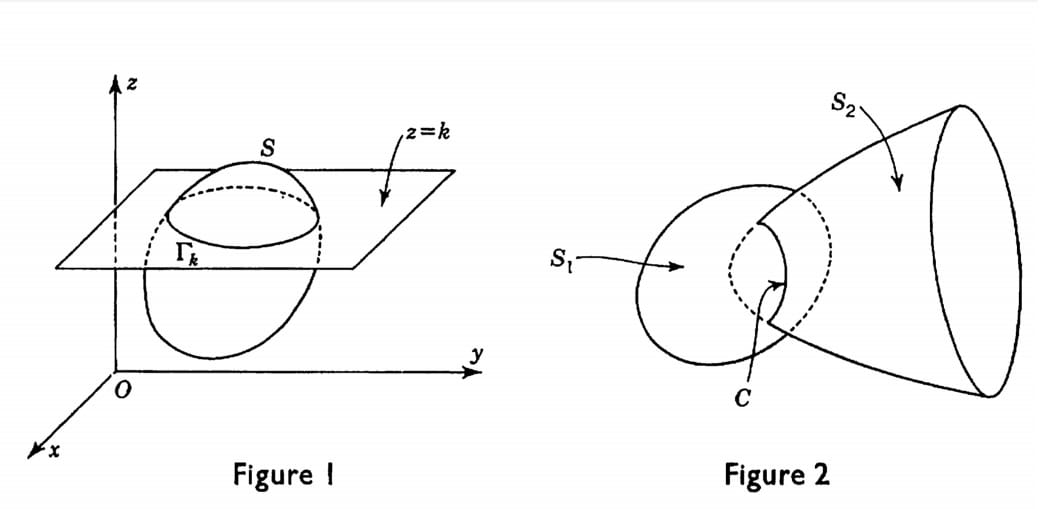
\includegraphics[scale=0.45]{Images/surfaceSection1.jpeg}
	\caption{Ejemplo de Curva en Superficie}
	\label{curveSurface}
\end{figure}

Esta idea puede ser facilmente generalizada simplemente tomando dos superficies que se intersectan, la curva de intersección es el análogo de $\Lambda _k$ en el ejemplo anterior. Esta idea esta representada en la "Figure 2" de \ref{curveSurface}. Matemáticamente hablando, la curva $C$ es conformada por todos aquellos puntos que cumplen las ecuaciones de ambas superficies:
	$$f(x,y,z) = 0 \quad \quad g(x,y,z) = 0$$
Dicha curva se puede representar por medio de sus ecuaciones paramétricas. Ahora, suponiendo que la curva $C$ esta sobre la superficie cuya ecuación es:
	$$F(x(t),y(t),z(t)) = 0$$
Derivando $F$ se tienen la relación:
	$$\pdv{F}{x} \dv{x}{t} + \pdv{F}{y} \dv{y}{t} + \pdv{F}{z} \dv{z}{t} = 0$$
De modo que la tangente a la curva es:
	$$\qty(\pdv{F}{x} , \pdv{F}{y} , \pdv{F}{z})$$
	
La ecuación del plano $\pi _1$ en el punto $P(x,y,z)$ y la superficie $S_1$ es:
	$$(X - x)\pdv{F}{x} + (Y - y)\pdv{F}{y} + (Z - z)\pdv{F}{z} = 0$$
Con $(X,Y,Z)$ es cualquier otro punto en el plano. Realizando lo mismo para la superficie $S_2$. Se tiene:
	$$(X - x)\pdv{G}{x} + (Y - y)\pdv{G}{y} + (Z - z)\pdv{G}{z} = 0$$
Y la intersección $L$ de los planos $\pi _1$ y $\pi _2$ en $P$ es tangente a la curva $C$. \\

Para visualizarlo de mejor manera, se tiene la siguiente figura:

\begin{figure}[H]
	\centering
	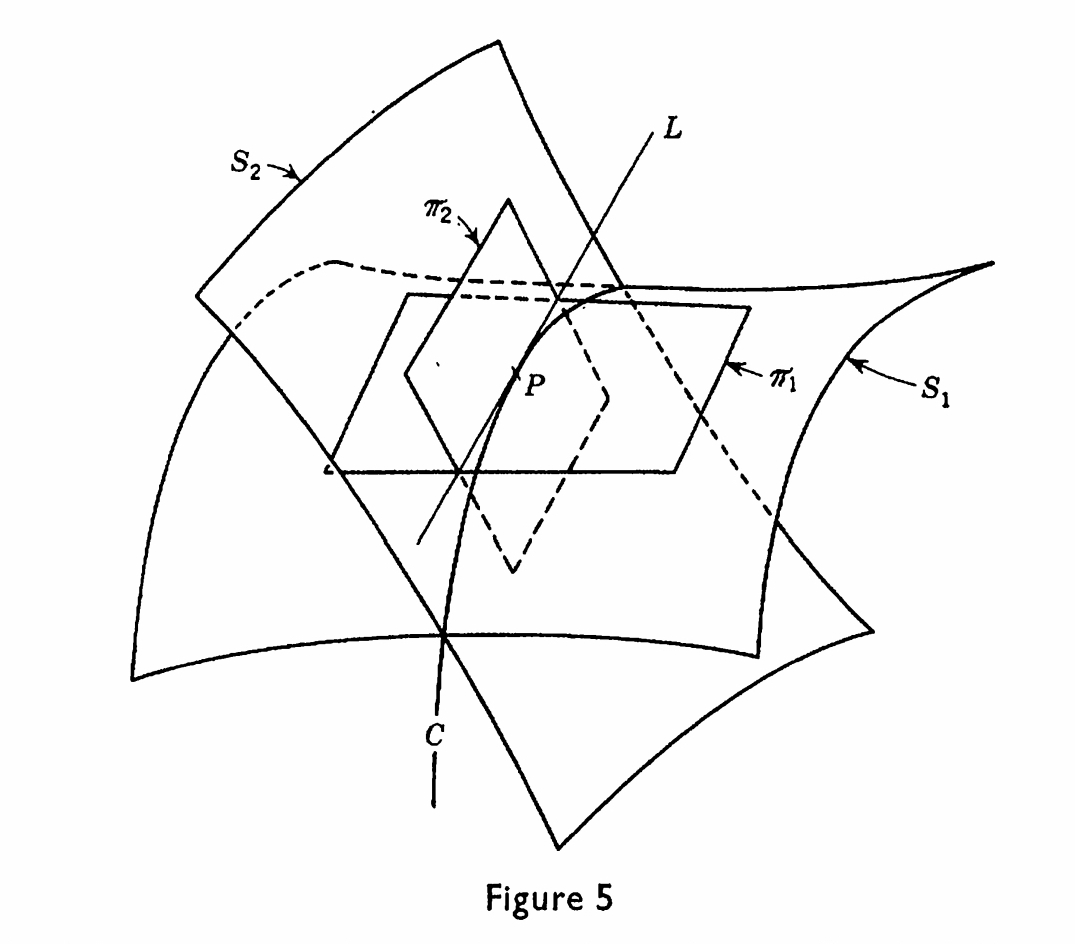
\includegraphics[scale=0.2]{Images/planesSection1.jpeg}
	\caption{Visualización de la Recta Tangente a la Curva}
	\label{planes}
\end{figure}

De las ecuaciones de los planos se tiene que las ecuaciones de la recta $L$ son:
	$$\frac{X - x}{\pdv{F}{y} \pdv{G}{z} - \pdv{F}{z} \pdv{G}{y}} = \frac{Y - y}{\pdv{F}{z} \pdv{G}{x} - \pdv{F}{x} \pdv{G}{z}} = \frac{Z - z}{\pdv{F}{x} \pdv{G}{y} - \pdv{F}{y} \pdv{G}{x}}$$

En otras palabras, las razones de dirección de la recta $L$ son:
	$$\Bigg\{ \pdv{(F,G)}{(y,z)} , \pdv{(F,G)}{(z,x)} , \pdv{(F,G)}{(x,y)} \Bigg\}$$


\subsection{Problemas Resueltos}


\section{Ecuaciones Diferenciales de Primer Orden y Primer Grado de Tres Variables}









































